\documentclass{article}
\usepackage[utf8]{inputenc}

\usepackage{amsfonts}
\usepackage{amssymb}
\usepackage{amsmath}
\usepackage{amsthm}
\usepackage{enumitem}
\usepackage{float}
\usepackage[clean]{svg}

\usepackage{graphicx}

\usepackage{bbold}
\usepackage{bm}
\usepackage{color}
\usepackage{hyperref}
\usepackage[margin=2.5cm]{geometry}

\usepackage{fancyhdr}

\usepackage[english]{babel}
\usepackage[T1]{fontenc}

\usepackage{tcolorbox}
\usepackage{fancyvrb}
\usepackage{scrextend}

\makeatletter

\makeatother

\begin{document}

% ==============================================================================

\title{High-Dimensional Statistics}								% Title
\author{Romain LAMBERMONT, Arthur LOUIS}								% Author
\date{\today}						% Date

\makeatletter
\let\thetitle\@title
\let\theauthor\@author
\let\thedate\@date
\makeatother

\pagestyle{fancy}
\fancyhf{}
\rhead{\theauthor}
\lhead{\thetitle}
\cfoot{\thepage}

\begin{titlepage}
 \centering
 \vspace*{0.5 cm}
 \includegraphics[scale = 0.7]{figs/facsa.png}\\[1.0 cm]	% University Logo
 \textsc{\LARGE \newline\newline Faculty of Applied Science}\\[2.0 cm]	% University Name
 \textsc{\Large MATH2021-1 High-dimensional statistics}\\[0.5 cm]				% Course Code
 \rule{\linewidth}{0.2 mm} \\[0.4 cm]
 {\huge \bfseries Project 1 : Exploratory Data Analysis}\\
 \rule{\linewidth}{0.2 mm} \\[1.5 cm]

 \begin{minipage}{0.5\textwidth}
 	\begin{flushleft} \large
 		\emph{Teacher :}\\
 		Gentiane HAESBROECK\\
    \vspace{0.5cm}
 		\end{flushleft}
 		\end{minipage}~
 		\begin{minipage}{0.4\textwidth}

 		\begin{flushright} \large
 		\emph{Group :} \\
    Romain LAMBERMONT\\
    Arthur LOUIS\\
      
 	\end{flushright}

 \end{minipage}\\[2 cm]
 \thedate
\end{titlepage}

% ==============================================================================
\thispagestyle{empty}
\tableofcontents
\listoffigures
\listoftables
\pagebreak
\setcounter{page}{1}

\subsection{Discussion on the data}
The data we used in this project is a subset of the data collected by the ENEA (National Agency for New Technologies, Energy and Sustainable Economic Development)
alonside a road in a polluted area of Italy. This dataset is available on the UCI repository\footnote{\href{https://archive.ics.uci.edu/ml/datasets/air+quality}{https://archive.ics.uci.edu/ml/datasets/air+quality}}. The data was harvested using a multicensor device and reference analyzers. The data was collected between March 2004 and February 2005.

There are 5 couples of variables in the dataset, each couple is composed of a variable measured by the reference analyzer and the corresponding variable measured by the multicensor device.
The values represent the hourly average concentration of each variable. In addition to the variables couples, we have 3 other variables representing the temperature and the humidity (both relative and absolute).
The different values are stored in the following columns of our dataset :
\begin{itemize}
\item \texttt{CO(GT)} : concentration of CO in the air (in mg/m$^3$)
\item \texttt{PT08.S1(C0)} : average sensor response (nominally CO targeted)
\item \texttt{NMHC(GT)} : concentration of non-methane hydrocarbons in the air (in $\mu$g/m$^3$)
\item \texttt{C6H6(GT)} : concentration of benzene in the air (in $\mu$g/m$^3$)
\item \texttt{PT08.S2(NMHC)} : average sensor response (nominally NMHC targeted)
\item \texttt{NOx(GT)} : concentration of NOx in the air (in parts per billion)
\item \texttt{PT08.S3(NOx)} : average sensor response (nominally NOx targeted)
\item \texttt{NO2(GT)} : concentration of NO$_2$ in the air (in $\mu$g/m$^3$)
\item \texttt{PT08.S4(NO2)} : average sensor response (nominally NO$_2$ targeted)
\item \texttt{PT08.S5(O3)} : average sensor response (nominally O$_3$ targeted)
\item \texttt{T} : temperature (in $^{\circ}$C)
\item \texttt{RH} : relative humidity (in $\%$)
\item \texttt{AH} : absolute humidity
\end{itemize}

On top of that, we created a binary indicator per variable measured by the reference analyzers which is equal to 1 when the measured value is above the median of the variable and 0 otherwise.
The binary values are stored in the following columns :

\begin{itemize}
  \item \texttt{HIGH\_CO} : binary indicator for CO (above/under median)
  \item \texttt{HIGH\_NMHC} : binary indicator for NMHC (above/under median)
  \item \texttt{HIGH\_C6H6} : binary indicator for benzene (above/under median)
  \item \texttt{HIGH\_NOx} : binary indicator for NOx (above/under median)
  \item \texttt{HIGH\_NO2} : binary indicator for NO2 (above/under median)
\end{itemize}

\subsection{Link between the variables}
The values for each couple are obviously going to be quite correlated, as they are measuring the same thing.
Furthermore, the values for the binary indicators are going to be highly correlated with the values of the corresponding measurements from the reference analyzers (as the binary indicator is equal to 1 when the value is above the median and 0 otherwise).

\section{Information about missing data}
We have a total of $2.1\%$ of missing values but this number is overestimated because the binary indicators are taken into account. The real ratio is $1.7\%$
without this indicators.
The missing values are due to hardware problems related to the measuring instruments
and to the fact that the data was collected in a real environment.

\begin{figure}[H]
\centering
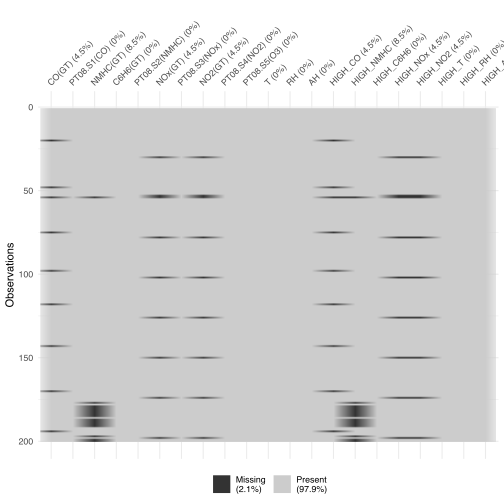
\includegraphics[width=0.5\textwidth]{figs/missing_values.png}
\caption{Missing data}
\label{fig:missing_data}
\end{figure}

\begin{figure}[H]
\centering
\includegraphics[width=0.5\textwidth]{figs/missing_values_heatmap.png}
\caption{Missing data heatmap}
\label{fig:missing_data_heatmap}
\end{figure}





\section{Exploratory data analysis}

\subsection{Statistical analysis}
\begin{table}[h]
  \centering
  \begin{tabular}{|c|c|c|c|c|c|c|}
    \hline
      & n & mean & sd & median & trimmed & mad\\
    \hline
    CO(GT) & 191 & 2.748691 & 1.596801 & 2.50 & 2.560784 & 1.33434\\
    \hline
    PT08.S1(CO) & 200 & 1339.000000 & 255.446559 & 1332.50 & 1328.356250 & 233.50950\\
    \hline
    NMHC(GT) & 183 & 160.158470 & 139.745774 & 122.00 & 138.448980 & 118.60800\\
    \hline
    C6H6(GT) & 200 & 12.254000 & 8.274006 & 11.05 & 11.318750 & 7.33887\\
    \hline
    PT08.S2(NMHC) & 200 & 1016.950000 & 281.940276 & 1017.50 & 1005.556250 & 278.72880\\
    \hline
    NOx(GT) & 191 & 175.842932 & 94.999980 & 161.00 & 168.830065 & 85.99080\\
    \hline
    PT08.S3(NOx) & 200 & 1003.195000 & 278.431170 & 945.00 & 976.950000 & 234.99210\\
    \hline
    NO2(GT) & 191 & 115.612565 & 34.357971 & 119.00 & 116.549020 & 35.58240\\
    \hline
    PT08.S4(NO2)9 & 200 & 1671.040000 & 305.901187 & 1622.50 & 1641.750000 & 237.21600\\
    \hline
  \end{tabular}

  \begin{tabular}{|c|c|c|c|c|c|c|}
    \hline
      & min & max & range & skew & kurtosis & se\\
    \hline
    CO(GT) & 0.5 & 8.1 & 7.6 & 1.0755547 & 0.9704424 & 0.1155405\\
    \hline
    PT08.S1(CO) & 831.0 & 2040.0 & 1209.0 & 0.3506958 & -0.0955406 & 18.0627994\\
    \hline
    NMHC(GT) & 7.0 & 685.0 & 678.0 & 1.3200143 & 1.4422105 & 10.3303049\\
    \hline
    C6H6(GT) & 1.0 & 39.2 & 38.2 & 1.0086394 & 0.8567735 & 0.5850606\\
    \hline
    PT08.S2(NMHC) & 501.0 & 1754.0 & 1253.0 & 0.3211184 & -0.3339212 & 19.9361881\\
    \hline
    NOx(GT) & 16.0 & 478.0 & 462.0 & 0.6699740 & -0.0263597 & 6.8739573\\
    \hline
    PT08.S3(NOx) & 537.0 & 1918.0 & 1381.0 & 0.9745243 & 0.9172654 & 19.6880569\\
    \hline
    NO2(GT) & 28.0 & 194.0 & 166.0 & -0.2179968 & -0.4405303 & 2.4860555\\
    \hline
    PT08.S4(NO2) & 1134.0 & 2679.0 & 1545.0 & 0.9116828 & 0.7869557 & 21.6304804\\
    \hline
  \end{tabular}
\end{table}

\begin{table}[h]
  \centering
  \begin{tabular}{|c|c|c|c|c|c|c|}
    \hline
    & n & mean & sd & median & trimmed & mad\\
    \hline
    PT08.S5(O3) & 200 & 1233.2450000 & 389.2906253 & 1204.5000 & 1222.0375000 & 384.734700\\
    \hline
    T & 200 & 15.1965000 & 5.5702402 & 14.3000 & 14.8068750 & 5.189100\\
    \hline
    RH & 200 & 49.8030000 & 15.1352426 & 53.9000 & 50.6387500 & 15.270780\\
    \hline
    AH & 200 & 0.8085450 & 0.1059962 & 0.8125 & 0.8092338 & 0.104375\\
    \hline
    HIGH\_CO & 191 & 0.7225131 & 0.4489355 & 1.0000 & 0.7777778 & 0.000000\\
    \hline
    HIGH\_NMHC & 183 & 0.9945355 & 0.0739221 & 1.0000 & 1.0000000 & 0.000000\\
    \hline
    HIGH\_C6H6 & 200 & 0.6500000 & 0.4781665 & 1.0000 & 0.6875000 & 0.000000\\
    \hline
    HIGH\_NOx & 191 & 0.9947644 & 0.0723575 & 1.0000 & 1.0000000 & 0.000000\\
    \hline
    HIGH\_NO2 & 191 & 0.5968586 & 0.4918179 & 1.0000 & 0.6209150 & 0.000000\\
    \hline
  \end{tabular}
  
  \begin{tabular}{|c|c|c|c|c|c|c|}
    \hline
    & min & max & range & skew & kurtosis & se\\
    \hline
    PT08.S5(O3) & 384.0000 & 2359.0000 & 1975.0000 & 0.2942286 & -0.1157893 & 27.5270041\\
    \hline
    T & 6.1000 & 29.3000 & 23.2000 & 0.6005822 & -0.4670720 & 0.3938755\\
    \hline
    RH & 14.9000 & 81.1000 & 66.2000 & -0.4375140 & -0.8600569 & 1.0702233\\
    \hline
    AH & 0.5237 & 1.0945 & 0.5708 & 0.0279583 & -0.2727186 & 0.0074951\\
    \hline
    HIGH\_CO  & 0.0000 & 1.0000 & 1.0000 & -0.9861019 & -1.0329289 & 0.0324838\\
    \hline
    HIGH\_NMHC & 0.0000 & 1.0000 & 1.0000 & -13.3067908 & 176.0326973 & 0.0054645\\
    \hline
    HIGH\_C6H6 & 0.0000 & 1.0000 & 1.0000 & -0.6242595 & -1.6183168 & 0.0338115\\
    \hline
    HIGH\_NOx & 0.0000 & 1.0000 & 1.0000 & -13.6039602 & 184.0313314 & 0.0052356\\
    \hline
    HIGH\_NO2 & 0.0000 & 1.0000 & 1.0000 & -0.3918179 & -1.8561145 & 0.0355867\\
    \hline
  \end{tabular}  

  \caption{Summary statistics}
\end{table}


\begin{figure}[H]
  \centering
  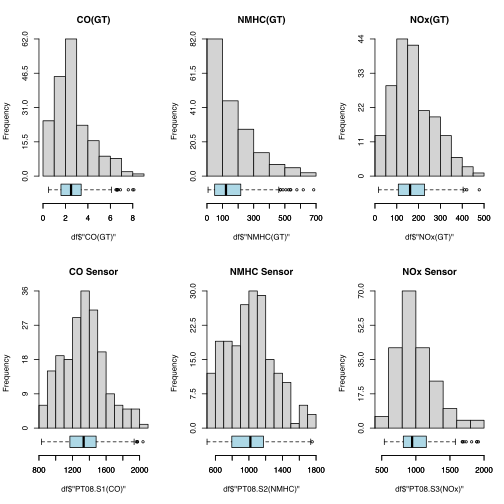
\includegraphics[width=0.7\textwidth]{figs/summary_1.png}
\end{figure}

\begin{figure}[H]
  \centering
  \includegraphics[width=0.7\textwidth]{figs/summary_2.png}
\end{figure}

\begin{figure}[H]
  \centering
  \includegraphics[width=0.5\textwidth]{figs/summary_3.png}
  \label{fig:summary}
  \caption{Summary of the data}
\end{figure}


\subsection{Correlation structure of the data}
\begin{figure}[H]
  \centering
  \includegraphics[width=0.5\textwidth]{figs/corr.png}
  \caption{Correlation matrix}
  \label{fig:corr}
\end{figure}

\begin{figure}[H]
  \centering
  \includegraphics[width=0.5\textwidth]{figs/scatter_matrix.png}
  \caption{Scatter matrix}
  \label{fig:scatter_matrix}
\end{figure}

%% analyze correlation
As can be seen in the two previous figures, the 10 first variables are correlated all together and the next 2 variables are also correlated together. The absloute humidity is isolated from the rest. This is a first clue that we can use to reduce the dimension of the data. We will use the PCA to reduce the dimension of the data.
The only variable collected by the sensors that is not correlated in the same with the others comes from the NOx sensor. Indeed, we can clearly dark red spot in the first figure and a linear relation in the other way on the second.

The variables relative to the humidity and temperature are much less correlated with the sensors varibles but much more within themselves. We can thus clearly see two groups of variables in the correlation matrix.

\subsection{Outlying observations using Mahalanobis distance}
\begin{figure}[H]
  \centering
  \includegraphics[width=0.5\textwidth]{figs/outliers.png}
  \caption{Mahalanobis distance outlier detection}
  \label{fig:mahalanobis}
\end{figure}

Using the \verb|outlier| function from \verb|pscyh| package, we can clearly distinguish the outliers from the dataset, which are the points that are not close to eachother.

\subsection{Choice between PCA and t-SNE}
%% TODO

\subsection{2D plot of the data}
%% TODO

\end{document}\documentclass{article}
\usepackage[utf8]{inputenc}

\usepackage{amsfonts}
\usepackage{amssymb}
\usepackage{amsmath}
\usepackage{amsthm}
\usepackage{enumitem}

\usepackage{graphicx}

\usepackage{bbold}
\usepackage{bm}
\usepackage{color}
\usepackage{hyperref}
\usepackage[margin=2.5cm]{geometry}

\usepackage{fancyhdr}

\usepackage[english]{babel}
\usepackage[T1]{fontenc}

\usepackage{tcolorbox}
\usepackage{fancyvrb}
\usepackage{scrextend}

\makeatletter

\makeatother

\begin{document}

% ==============================================================================

\title{High-Dimensional Statistics}								% Title
\author{Romain LAMBERMONT, Arthur LOUIS}								% Author
\date{\today}						% Date

\makeatletter
\let\thetitle\@title
\let\theauthor\@author
\let\thedate\@date
\makeatother

\pagestyle{fancy}
\fancyhf{}
\rhead{\theauthor}
\lhead{\thetitle}
\cfoot{\thepage}

\begin{titlepage}
 \centering
 \vspace*{0.5 cm}
 \includegraphics[scale = 0.7]{figs/facsa.png}\\[1.0 cm]	% University Logo
 \textsc{\LARGE \newline\newline Faculty of Applied Science}\\[2.0 cm]	% University Name
 \textsc{\Large MATH2021-1 High-dimensional statistics}\\[0.5 cm]				% Course Code
 \rule{\linewidth}{0.2 mm} \\[0.4 cm]
 {\huge \bfseries Project 1 : Exploratory Data Analysis}\\
 \rule{\linewidth}{0.2 mm} \\[1.5 cm]

 \begin{minipage}{0.5\textwidth}
 	\begin{flushleft} \large
 		\emph{Teacher :}\\
 		Gentiane HAESBROECK\\
    \vspace{0.5cm}
 		\end{flushleft}
 		\end{minipage}~
 		\begin{minipage}{0.4\textwidth}

 		\begin{flushright} \large
 		\emph{Group :} \\
    Romain LAMBERMONT\\
    Arthur LOUIS\\
      
 	\end{flushright}

 \end{minipage}\\[2 cm]
 \thedate
\end{titlepage}

% ==============================================================================
\thispagestyle{empty}
\tableofcontents
\listoffigures
\listoftables
\pagebreak
\setcounter{page}{1}

\subsection{Discussion on the data}
The data we used in this project is a subset of the data collected by the ENEA (National Agency for New Technologies, Energy and Sustainable Economic Development)
alonside a road in a polluted area of Italy. This dataset is available on the UCI repository\footnote{\href{https://archive.ics.uci.edu/ml/datasets/air+quality}{https://archive.ics.uci.edu/ml/datasets/air+quality}}. The data was harvested using a multicensor device and reference analyzers. The data was collected between March 2004 and February 2005.

There are 5 couples of variables in the dataset, each couple is composed of a variable measured by the reference analyzer and the corresponding variable measured by the multicensor device.
The values represent the hourly average concentration of each variable. In addition to the variables couples, we have 3 other variables representing the temperature and the humidity (both relative and absolute).
The different values are stored in the following columns of our dataset :
\begin{itemize}
\item \texttt{CO(GT)} : concentration of CO in the air (in mg/m$^3$)
\item \texttt{PT08.S1(C0)} : average sensor response (nominally CO targeted)
\item \texttt{NMHC(GT)} : concentration of non-methane hydrocarbons in the air (in $\mu$g/m$^3$)
\item \texttt{C6H6(GT)} : concentration of benzene in the air (in $\mu$g/m$^3$)
\item \texttt{PT08.S2(NMHC)} : average sensor response (nominally NMHC targeted)
\item \texttt{NOx(GT)} : concentration of NOx in the air (in parts per billion)
\item \texttt{PT08.S3(NOx)} : average sensor response (nominally NOx targeted)
\item \texttt{NO2(GT)} : concentration of NO$_2$ in the air (in $\mu$g/m$^3$)
\item \texttt{PT08.S4(NO2)} : average sensor response (nominally NO$_2$ targeted)
\item \texttt{PT08.S5(O3)} : average sensor response (nominally O$_3$ targeted)
\item \texttt{T} : temperature (in $^{\circ}$C)
\item \texttt{RH} : relative humidity (in $\%$)
\item \texttt{AH} : absolute humidity
\end{itemize}

On top of that, we created a binary indicator per variable measured by the reference analyzers which is equal to 1 when the measured value is above the median of the variable and 0 otherwise.
The binary values are stored in the following columns :

\begin{itemize}
  \item \texttt{HIGH\_CO} : binary indicator for CO (above/under median)
  \item \texttt{HIGH\_NMHC} : binary indicator for NMHC (above/under median)
  \item \texttt{HIGH\_C6H6} : binary indicator for benzene (above/under median)
  \item \texttt{HIGH\_NOx} : binary indicator for NOx (above/under median)
  \item \texttt{HIGH\_NO2} : binary indicator for NO2 (above/under median)
\end{itemize}

\subsection{Link between the variables}
The values for each couple are obviously going to be quite correlated, as they are measuring the same thing.
Furthermore, the values for the binary indicators are going to be highly correlated with the values of the corresponding measurements from the reference analyzers (as the binary indicator is equal to 1 when the value is above the median and 0 otherwise).

\section{Information about missing data}
We have a total of $2.1\%$ of missing values but this number is overestimated because the binary indicators are taken into account. The real ratio is $1.7\%$
without this indicators.
The missing values are due to hardware problems related to the measuring instruments
and to the fact that the data was collected in a real environment.

\begin{figure}[H]
\centering
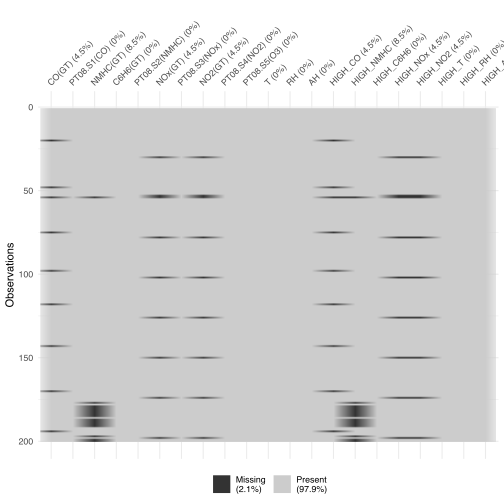
\includegraphics[width=0.5\textwidth]{figs/missing_values.png}
\caption{Missing data}
\label{fig:missing_data}
\end{figure}

\begin{figure}[H]
\centering
\includegraphics[width=0.5\textwidth]{figs/missing_values_heatmap.png}
\caption{Missing data heatmap}
\label{fig:missing_data_heatmap}
\end{figure}





\section{Exploratory data analysis}

\subsection{Statistical analysis}
\begin{table}[h]
  \centering
  \begin{tabular}{|c|c|c|c|c|c|c|}
    \hline
      & n & mean & sd & median & trimmed & mad\\
    \hline
    CO(GT) & 191 & 2.748691 & 1.596801 & 2.50 & 2.560784 & 1.33434\\
    \hline
    PT08.S1(CO) & 200 & 1339.000000 & 255.446559 & 1332.50 & 1328.356250 & 233.50950\\
    \hline
    NMHC(GT) & 183 & 160.158470 & 139.745774 & 122.00 & 138.448980 & 118.60800\\
    \hline
    C6H6(GT) & 200 & 12.254000 & 8.274006 & 11.05 & 11.318750 & 7.33887\\
    \hline
    PT08.S2(NMHC) & 200 & 1016.950000 & 281.940276 & 1017.50 & 1005.556250 & 278.72880\\
    \hline
    NOx(GT) & 191 & 175.842932 & 94.999980 & 161.00 & 168.830065 & 85.99080\\
    \hline
    PT08.S3(NOx) & 200 & 1003.195000 & 278.431170 & 945.00 & 976.950000 & 234.99210\\
    \hline
    NO2(GT) & 191 & 115.612565 & 34.357971 & 119.00 & 116.549020 & 35.58240\\
    \hline
    PT08.S4(NO2)9 & 200 & 1671.040000 & 305.901187 & 1622.50 & 1641.750000 & 237.21600\\
    \hline
  \end{tabular}

  \begin{tabular}{|c|c|c|c|c|c|c|}
    \hline
      & min & max & range & skew & kurtosis & se\\
    \hline
    CO(GT) & 0.5 & 8.1 & 7.6 & 1.0755547 & 0.9704424 & 0.1155405\\
    \hline
    PT08.S1(CO) & 831.0 & 2040.0 & 1209.0 & 0.3506958 & -0.0955406 & 18.0627994\\
    \hline
    NMHC(GT) & 7.0 & 685.0 & 678.0 & 1.3200143 & 1.4422105 & 10.3303049\\
    \hline
    C6H6(GT) & 1.0 & 39.2 & 38.2 & 1.0086394 & 0.8567735 & 0.5850606\\
    \hline
    PT08.S2(NMHC) & 501.0 & 1754.0 & 1253.0 & 0.3211184 & -0.3339212 & 19.9361881\\
    \hline
    NOx(GT) & 16.0 & 478.0 & 462.0 & 0.6699740 & -0.0263597 & 6.8739573\\
    \hline
    PT08.S3(NOx) & 537.0 & 1918.0 & 1381.0 & 0.9745243 & 0.9172654 & 19.6880569\\
    \hline
    NO2(GT) & 28.0 & 194.0 & 166.0 & -0.2179968 & -0.4405303 & 2.4860555\\
    \hline
    PT08.S4(NO2) & 1134.0 & 2679.0 & 1545.0 & 0.9116828 & 0.7869557 & 21.6304804\\
    \hline
  \end{tabular}
\end{table}

\begin{table}[h]
  \centering
  \begin{tabular}{|c|c|c|c|c|c|c|}
    \hline
    & n & mean & sd & median & trimmed & mad\\
    \hline
    PT08.S5(O3) & 200 & 1233.2450000 & 389.2906253 & 1204.5000 & 1222.0375000 & 384.734700\\
    \hline
    T & 200 & 15.1965000 & 5.5702402 & 14.3000 & 14.8068750 & 5.189100\\
    \hline
    RH & 200 & 49.8030000 & 15.1352426 & 53.9000 & 50.6387500 & 15.270780\\
    \hline
    AH & 200 & 0.8085450 & 0.1059962 & 0.8125 & 0.8092338 & 0.104375\\
    \hline
    HIGH\_CO & 191 & 0.7225131 & 0.4489355 & 1.0000 & 0.7777778 & 0.000000\\
    \hline
    HIGH\_NMHC & 183 & 0.9945355 & 0.0739221 & 1.0000 & 1.0000000 & 0.000000\\
    \hline
    HIGH\_C6H6 & 200 & 0.6500000 & 0.4781665 & 1.0000 & 0.6875000 & 0.000000\\
    \hline
    HIGH\_NOx & 191 & 0.9947644 & 0.0723575 & 1.0000 & 1.0000000 & 0.000000\\
    \hline
    HIGH\_NO2 & 191 & 0.5968586 & 0.4918179 & 1.0000 & 0.6209150 & 0.000000\\
    \hline
  \end{tabular}
  
  \begin{tabular}{|c|c|c|c|c|c|c|}
    \hline
    & min & max & range & skew & kurtosis & se\\
    \hline
    PT08.S5(O3) & 384.0000 & 2359.0000 & 1975.0000 & 0.2942286 & -0.1157893 & 27.5270041\\
    \hline
    T & 6.1000 & 29.3000 & 23.2000 & 0.6005822 & -0.4670720 & 0.3938755\\
    \hline
    RH & 14.9000 & 81.1000 & 66.2000 & -0.4375140 & -0.8600569 & 1.0702233\\
    \hline
    AH & 0.5237 & 1.0945 & 0.5708 & 0.0279583 & -0.2727186 & 0.0074951\\
    \hline
    HIGH\_CO  & 0.0000 & 1.0000 & 1.0000 & -0.9861019 & -1.0329289 & 0.0324838\\
    \hline
    HIGH\_NMHC & 0.0000 & 1.0000 & 1.0000 & -13.3067908 & 176.0326973 & 0.0054645\\
    \hline
    HIGH\_C6H6 & 0.0000 & 1.0000 & 1.0000 & -0.6242595 & -1.6183168 & 0.0338115\\
    \hline
    HIGH\_NOx & 0.0000 & 1.0000 & 1.0000 & -13.6039602 & 184.0313314 & 0.0052356\\
    \hline
    HIGH\_NO2 & 0.0000 & 1.0000 & 1.0000 & -0.3918179 & -1.8561145 & 0.0355867\\
    \hline
  \end{tabular}  

  \caption{Summary statistics}
\end{table}


\begin{figure}[H]
  \centering
  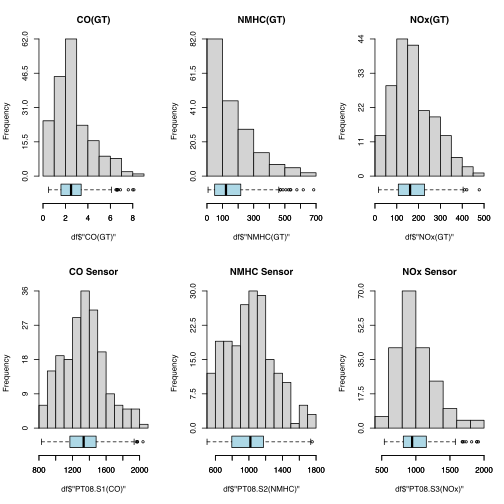
\includegraphics[width=0.7\textwidth]{figs/summary_1.png}
\end{figure}

\begin{figure}[H]
  \centering
  \includegraphics[width=0.7\textwidth]{figs/summary_2.png}
\end{figure}

\begin{figure}[H]
  \centering
  \includegraphics[width=0.5\textwidth]{figs/summary_3.png}
  \label{fig:summary}
  \caption{Summary of the data}
\end{figure}


\subsection{Correlation structure of the data}
\begin{figure}[H]
  \centering
  \includegraphics[width=0.5\textwidth]{figs/corr.png}
  \caption{Correlation matrix}
  \label{fig:corr}
\end{figure}

\begin{figure}[H]
  \centering
  \includegraphics[width=0.5\textwidth]{figs/scatter_matrix.png}
  \caption{Scatter matrix}
  \label{fig:scatter_matrix}
\end{figure}

%% analyze correlation
As can be seen in the two previous figures, the 10 first variables are correlated all together and the next 2 variables are also correlated together. The absloute humidity is isolated from the rest. This is a first clue that we can use to reduce the dimension of the data. We will use the PCA to reduce the dimension of the data.
The only variable collected by the sensors that is not correlated in the same with the others comes from the NOx sensor. Indeed, we can clearly dark red spot in the first figure and a linear relation in the other way on the second.

The variables relative to the humidity and temperature are much less correlated with the sensors varibles but much more within themselves. We can thus clearly see two groups of variables in the correlation matrix.

\subsection{Outlying observations using Mahalanobis distance}
\begin{figure}[H]
  \centering
  \includegraphics[width=0.5\textwidth]{figs/outliers.png}
  \caption{Mahalanobis distance outlier detection}
  \label{fig:mahalanobis}
\end{figure}

Using the \verb|outlier| function from \verb|pscyh| package, we can clearly distinguish the outliers from the dataset, which are the points that are not close to eachother.

\subsection{Choice between PCA and t-SNE}
%% TODO

\subsection{2D plot of the data}
%% TODO

\end{document}